\chapter{Motivation} \label{chapter:MOTIVATION}

In the Lively Kernel, programmers can create applications by manipulating and composing graphical parts.
This chapter demonstrates the development of such parts and related recovery needs by example.


\section{Part Development By Example}

To exemplify how developers work directly on objects in Lively, we will outline the process of adding a new feature to the Lively Kernel's Object Editor.

\begin{figure}[h]
    \centering
    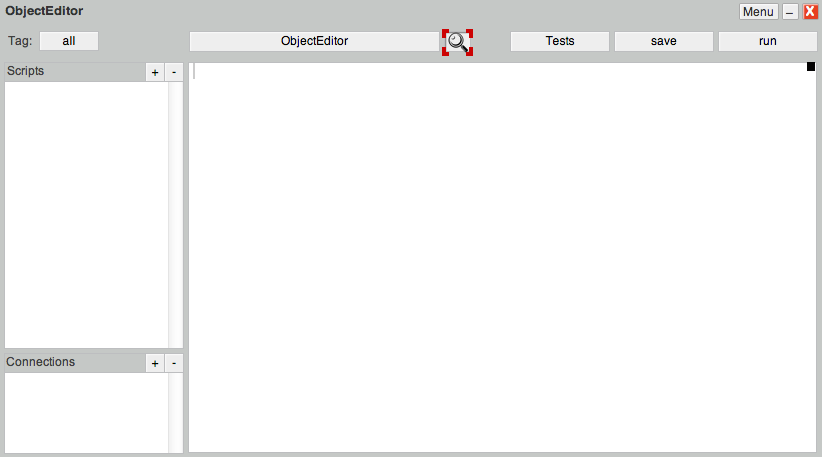
\includegraphics[width=\textwidth]{figures/3_motivation/1_magnifierButton.png}
    \caption{The Object Editor with its magnifier button highlighted with a red outline.}
    \label{fig:MagnifierButton}
\end{figure}

The editor itself has been been developed by composing and editing graphical objects.
For this reason, we do not adapt any source code modules to change the editor, but rather manipulate objects directly.
The new feature we add in this example is a magnifier button that can show the editor's current target.
Adding this feature requires to create and add a new button morph to the editor, as shown in Figure~\ref{fig:MagnifierButton}.

The magnifier button implements two features: First, when a programmer hovers over the button, the Object Editor's current target is highlighted through a rectangular overlay. Second, when a programmer clicks the button, the current target selection is revoked and the programmer can select the new target of the editor.
This example covers the first of these two behaviors, which is also shown in Figure~\ref{fig:MagnifierBehavior} for an Object Editor currently targeting the character of a game.

\begin{figure}[h]
    \centering
    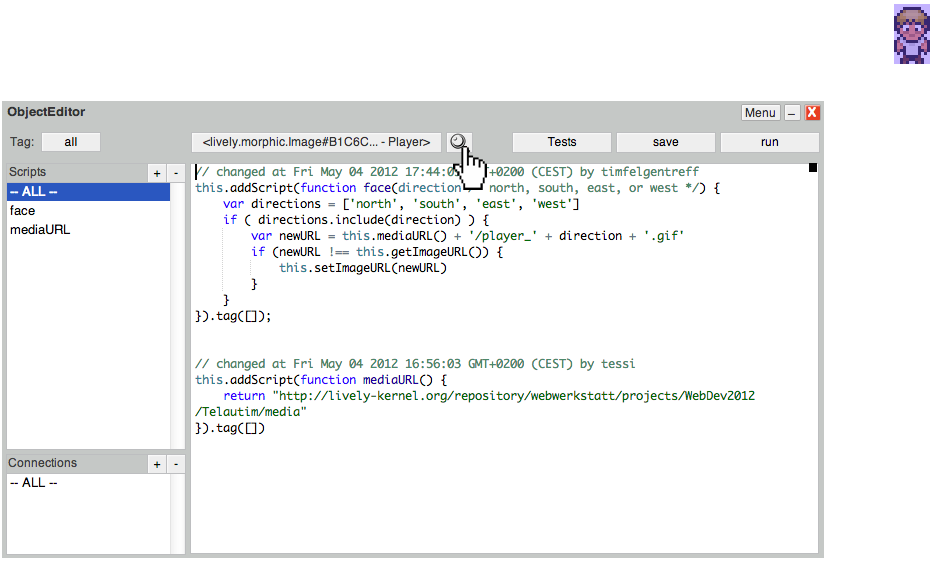
\includegraphics[width=0.8\textwidth]{figures/3_motivation/2_magnifierBehavior.png}
    \caption{Hovering the Object Editor's magnifier button highlights the current target object.}
    \label{fig:MagnifierBehavior}
\end{figure}

\paragraph{Manipulating the Button Morph}
Before we implement the button's behavior, we first create the button's visual appearance, as shown in Figure~\ref{fig:ButtonBuilding}.
A basic button, as visible in \circnum{1}, can be found in the Parts Bin repository.
We can use the button's halo buttons and, in particular, the resize tool in \circnum{2} to give the button a smaller and square extent.
Next, we can load an image showing a magnifier.
Using drag and drop we can add the image to the button, as done in \circnum{3}.
Dropping a morph onto another creates a parent-child relationship and structurally connects the two morphs.
That is, moving the button around will also move the image accordingly.
Saving will also persist both.
Subsequentely, we can add the result of these direct manipulations, visible in \circnum{4}, to the object editor.

\begin{figure}[h]
    \centering
    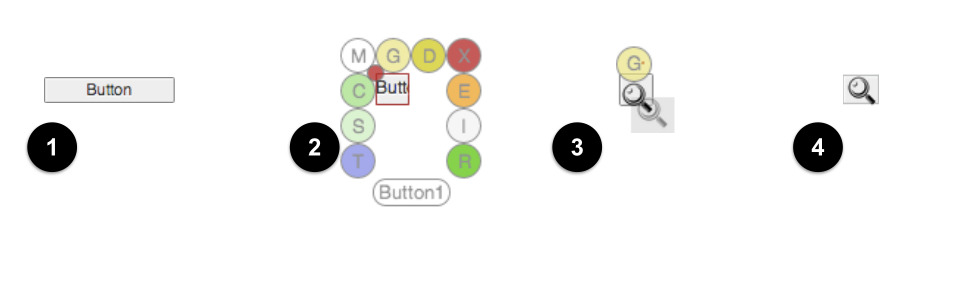
\includegraphics[width=\textwidth]{figures/3_motivation/3_buildingTheButton.png}
    \caption{Directly manipulating a button morph.}
    \label{fig:ButtonBuilding}
\end{figure}

All these changes are made directly to the state of objects: the button morph, the magnifier image morph, and the editor morph.\\
When programmers edit parts in this way, they often see the effects of their actions immediately.
For example, when adding the new button to the Object Editor, the button is visible at all times.
It is not necessary to run any code to check the resulting appearance.

\paragraph{Scripting the Button Morph}
Next, the magnifier button needs its behavior.
We add scripts to the button that lay a translucent rectangle over the current target.
The implementation of this could include the following: 
\begin{itemize}
    \item The button holds a semitransparent rectangle overlay.
    \item When the mouse enters the button (\lstinline{onMouseMove}), the button resizes and adds the rectangle to the world at the position of the target.
    \item When the mouse leaves the button (\lstinline{onMouseOut}), the button removes the rectangle again from the world.
\end{itemize}
 
When developing such scripts with an Object Editor, the editor allows to evaluate code in the context of its target.
So, when developers want to test a script or even just specific lines of code, they can often try the behavior directly with the actual target.


\section{Recovery Needs When Developing Parts}

While manipulating objects directly, developers might make changes that they later want to undo.

In the previous example we could, for example, make \emph{accidental changes}:

\begin{itemize}
    \item \textbf{Accidental changes to state}: We could accidentally grap and move a morph such as the new button and, thereby, change the carefully arranged layout. Similarly, we could close a morph such as the Object Editor, which contains the new button, and, thus, lose meaningful unsaved changes.
    \item \textbf{Accidental changes to scripts}: We could introduce a typographical error or accidentally remove a script. Moreover, we could introduce an error or a decrease in performance with an edit to ascript.
\end{itemize}

Besides these accidental changes, we could also make well-intentioned changes that nervertheless turn out to be \emph{inappropriate changes} later:

\begin{itemize}
    \item \textbf{Inappropriate changes through direct manipulation}: We could make many changes to the sizes, the positions, and the colors of morphs as, for example, when fine-tuning the visual appearance of an interface, only to decide later that a particular intermediate version was most appealing.
    \item \textbf{Inappropriate changes through scripts}: We could make a mistake in a workspace snippet that is intended to manipulate morph properties programmatically. Such a snippet can change any number of properties of many objects at once, so re-establishing a previous state would be a laborious task.
\end{itemize}

\paragraph{Explorative Script Evaluation}
Potentially undesirable changes might also be introduced when programmers explore the behavior of objects by evaluating scripts.
For example, the Object Editor always manipulates the scripts of a specific object and developers can evaluate code directly for that target object.
While such evaluation might help to understand the effects of particular code, it might also change the state of objects permanently.
A programmer could be working on the button's \lstinline{onMouseMove} script and could evaluate a few lines of code to quickly test it.
These lines, as shown in Figure~\ref{fig:onMouseOverScript}, would add the rectangle to the current target without regard to the conditions usually checked before.
Evaluating only the selected lines would also not set the state as done by the lines right below.
Thus, evaluating this selection allows to test the highlighting behavior, but leaves the system in a state that it would normally not be in.

\begin{figure}[h]
    \centering
    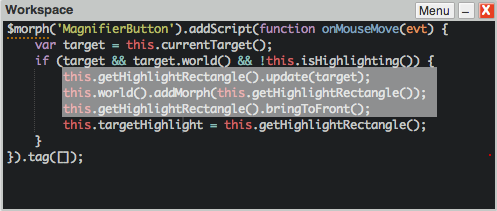
\includegraphics[width=0.7\textwidth]{figures/3_motivation/4_workspaceDoIt.png}
    \caption{The button's \lstinline{onMouseMove} script with a text selection.}
    \label{fig:onMouseOverScript}
\end{figure}

The given examples show that there are many situations in which developers might want to undo some of their operations.
In programming systems like the Lively Kernel, where programmers often work at runtime on objects, the development state consists of the state of objects.
Even classes and modules are objects in the Lively Kernel.
That is, changes are always made to objects.
More precisely, changes are always made to the \emph{state of objects} as even functions are also just properties of objects.

\begin{figure}[h]
    \centering
    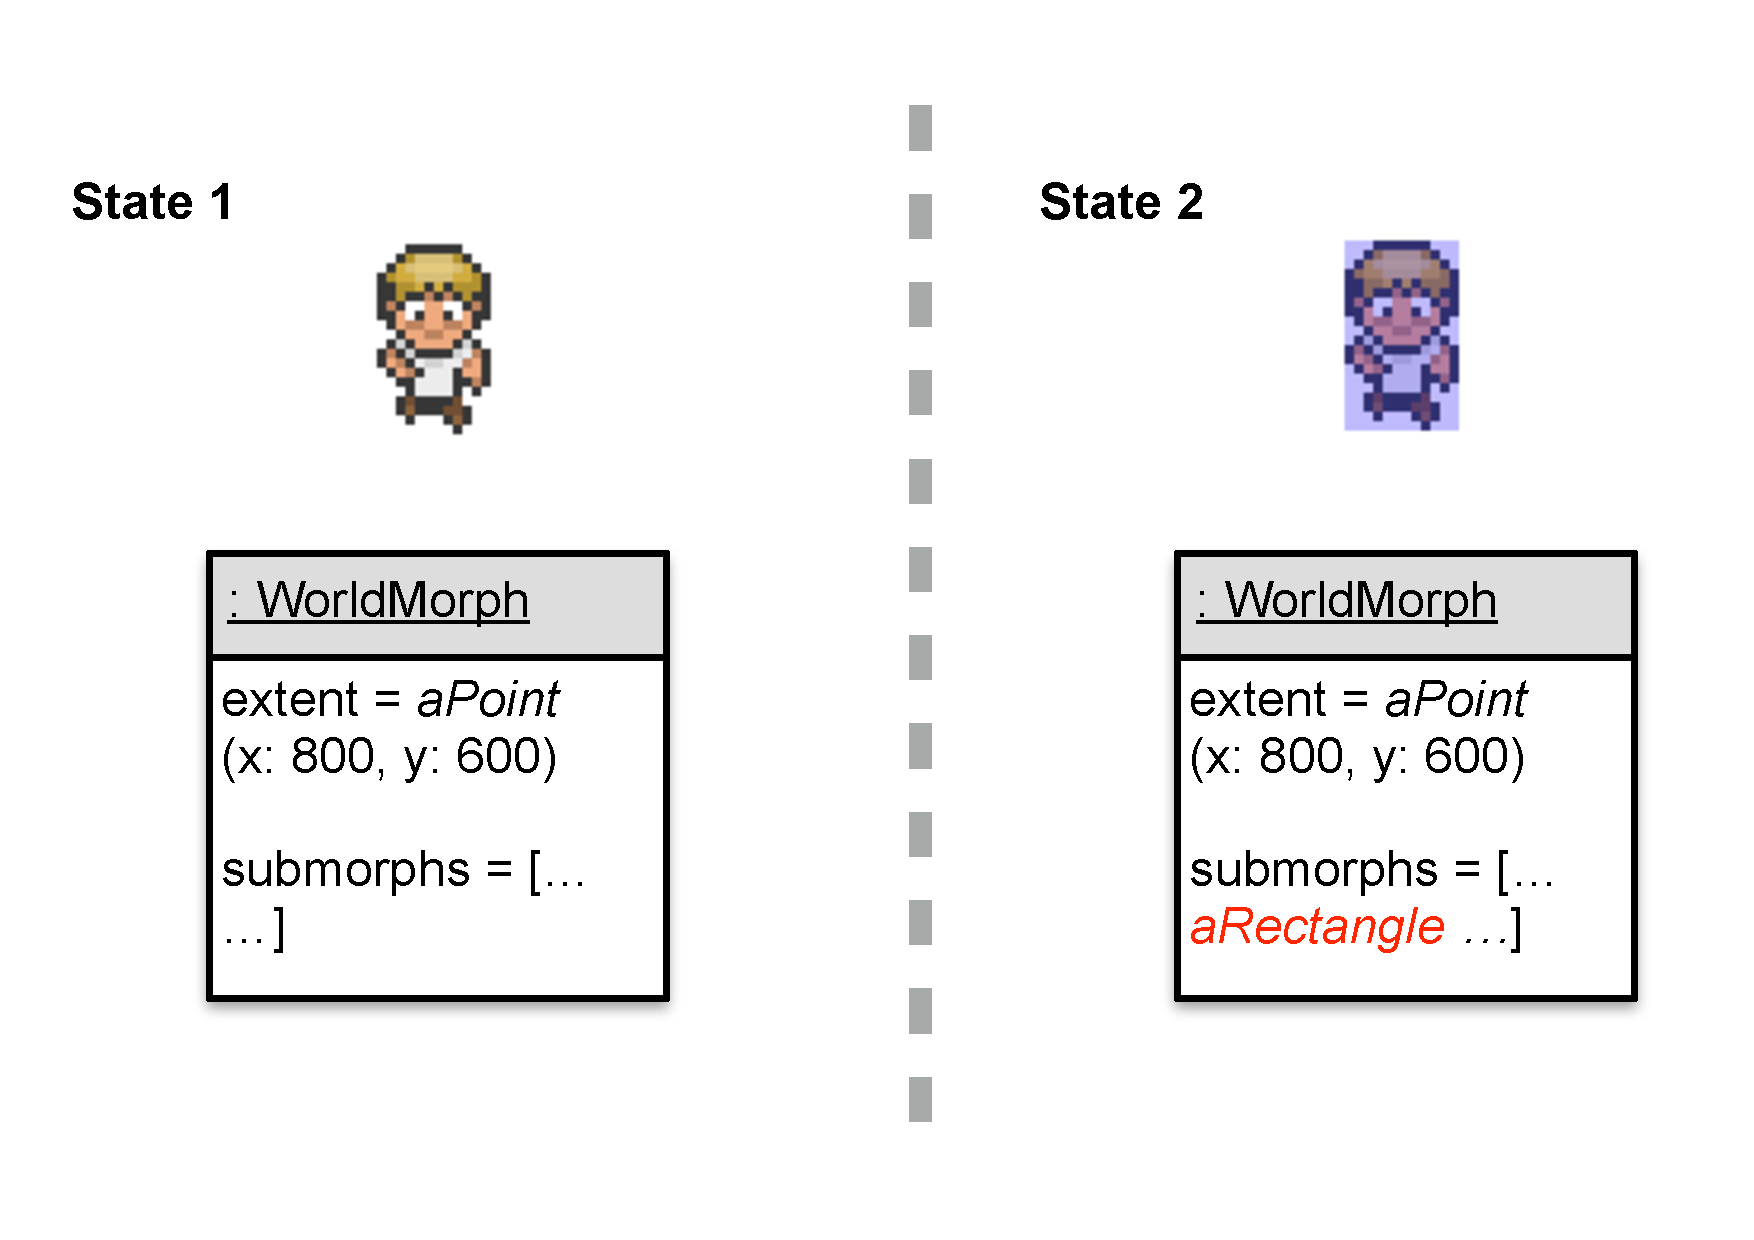
\includegraphics[width=0.7\textwidth]{figures/3_motivation/5_stateChanges.pdf}
    \caption{Adding a submorph changes the state of a morph.}
    \label{fig:changedCharacter}
\end{figure}

If, for example, the text selection in Figure~\ref{fig:onMouseOverScript} gets evaluated, the world object is changed.
In particular, its collection of submorphs is altered.
The world has now one more submorph, as shown in Figure~\ref{fig:changedCharacter}.

To undo the change and re-establish the previous version of the character, the world object needs to have its previous state.
The \lstinline{submorphs} property needs to be as it previously was.
Similarly, when the state of all objects is preserved and can be re-established on demand, previous development states can be recovered whenever recovery is necessary.
